% LSTM
\subsection{Probabilistic Neural Network Architecture}
Recently, recurrent architectures for time series regression have emerged that combine ridge functions with state vectors to create units with ``memory''. The most successful of these has been the long short-term memory architecture (LSTM), introduced by \cite{Hochreiter1997}. The LSTM cell, as its name implies, uses new input data with both the previous output and previous internal state to update its internal state and generate new output (Supplement, Text S6). This architecture has been applied to Dst forecasting by \cite{Gruet2018}, but, like all previous applications of neural networks to storm forecasting (summarized in the Supplement, Table S1), the network generated deterministic output with no prediction of forecast uncertainty.

\begin{figure}[htbp]
   \centering
   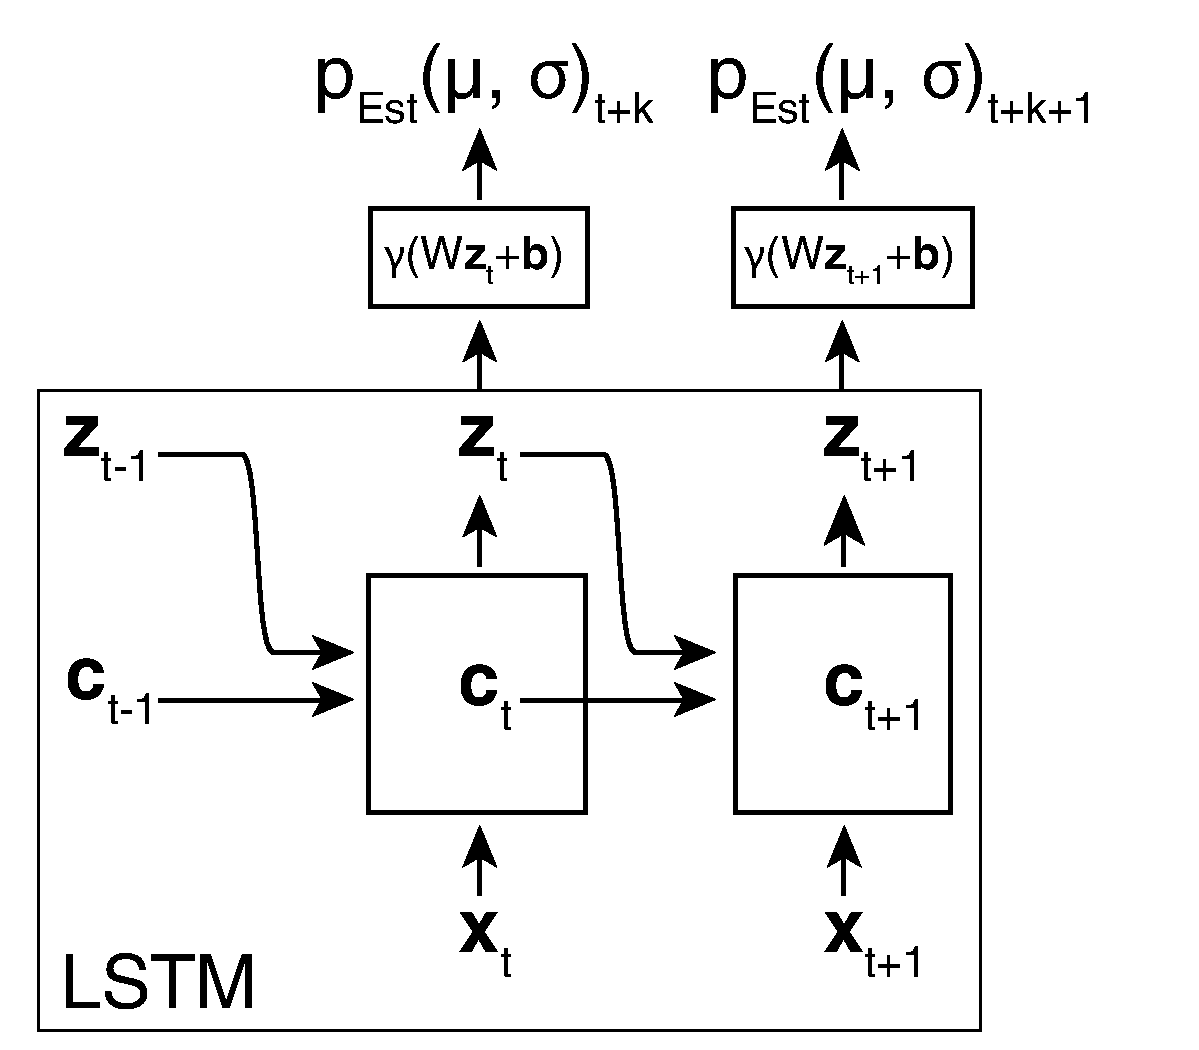
\includegraphics[width=0.7\textwidth]{figures/architecture_prob.pdf} % requires the graphicx package
   \caption{Schematic architecture for the deterministic network that learns parameters over an output distribution for Est. Our output distribution is a Gaussian. Two full time steps of network iteration are shown, with the portion of the network enclosing the LSTM cell labeled ``LSTM''.}
   \label{fig:architecture}
\end{figure}

We present an architecture (Figure~\ref{fig:architecture}) in which the NN learns to assess uncertainty in its own forecast, thereby generating probabilistic forecasts. The two basic layers utilized within this architecture are LSTM and dense layers. The former is described above, and the latter is an implementation of the so-called ``fully connected hidden layer'', which references the fact that each entry in $\mathbf{z}$ depends on all of the outputs from the preceding layer via $W$. That is, a dense layer that receives inputs $\mathbf{x} \in \mathbb{R}^n$ from a preceding network layer in turn generates an output vector $\mathbf{z} \in \mathbb{R}^m$ via the operation $\mathbf{z} = \gamma(W\,\mathbf{x} + \mathbf{b})$ with $W \in \mathbb{R}^{mxn}$ and $\mathbf{b} \in \mathbb{R}^m$, where $n$ is the dimensionality of the preceding hidden layer, $m$ is the dimensionality of the current hidden layer, and $\gamma(.)$ is a nonlinear activation function that acts element-wise. 

Inputs into our NN architecture are fed directly to an LSTM cell, and outputs from the LSTM cell are fed through a series of fully-connected hidden layers. The outputs from the last hidden layer are parameters for an output distribution over Est. We choose to use a Gaussian output distribution and compare other alternatives in the Supplement (Text S3). 

The simplest cost function in this probabilistic framework is precisely the output distribution itself evaluated as a likelihood of observed data $y$ (i.e., Est at some time $t+k$) with respect to the distribution parameters generated from the given input:
\begin{equation}
C(\mathbf{x}, y) = -\log p\left( y \vert \mu(W, \mathbf{b}, \mathbf{x}), \sigma(W, \mathbf{b}, \mathbf{x})\right) \label{eq:output}
\end{equation}
where the distribution parameters $\mu$ and $\sigma$ depend on the network weights and biases and can thus be differentiated against them. However, when learning two-parameter distributions, the parameter for scale often introduces leniency in the output distribution, allowing the network to expand uncertainty in its forecast rather than move its estimate for the center (see supplement Text S3). 

We found that utilizing a Gaussian output distribution with a regularized Gaussian likelihood as the cost function performed well for geomagnetic storm forecasting. Equation~\ref{eq:gaussian_mod} shows the form for this modified log-likelihood in which $\alpha\,(y-\mu)^2 + \beta\,\frac{1}{\sigma^2}$ are the terms that we have added, introducing $\alpha$ and $\beta$ as additional hyper-parameters. This regularization encourages the network to learn more reasonable estimates for $\mu$, offsetting the normalization by $\sigma^2$, while also allowing the user to further incentivize ($\beta > 0$) or penalize ($\beta < 0$) expanding forecast uncertainty.

\begin{equation}
    C_{\mathrm{Gaussian,\, regularized}}(y, \mu, \sigma) = \log\left(\sqrt{2\,\pi}\,\sigma \right) + \frac{\left(y-\mu \right)^2}{2\,\sigma^2} +  \alpha\,\left(y-\mu \right)^2 + \beta\,\frac{1}{\sigma^2} \label{eq:gaussian_mod}
\end{equation}
Other approaches have been formulated for learning uncertainty via neural networks, such as Bayes-by-Backprop \citep{Blundell2015}, which represents uncertainty in the network weights rather than in its output. Our implementation of this approach was not useful for storm forecasting (Supplement Text S2).

For all implementations, training, and testing of neural networks, we use Python wrappers for the learning framework TensorFlow \citep{tensorflow}. This framework is capable of representing neurons and the functional operations relating them as well as numerically computing the relevant gradients to train the network. TensorFlow provides an implementation of the high level deep learning Keras API (\url{https://keras.io/}), which allows for modular construction of networks from the layers described above. We also make use of the recently introduced TensorFlow Probability library, which provides a straightforward means of adding probability distributions as layers, allowing outputs from previous layers to be used as parameters for the distribution layers. These layers are compiled into a model that contains all the operations of the entire network as well as the particular cost functions and optimizers that dictate the learning process for given training inputs and outputs. We use the Adam optimizer for gradient update steps \citep{Kingma2014adam}. All neural network configuration and training parameters are listed in Supplement Text S4.


%%
%% OUTPUT DATA
%%
\subsection{Output Data}
Most geomagnetic storm forecasting thus far has emphasized prediction of Dst. However, Dst is actually a sum of internal and external components (Equation~\ref{eq:dst}), and the internal component, Ist, is generated by currents induced in Earth's subsurface by variation in the external component, Est \citep{Maus2004} (Equation~\ref{eq:ist}),
\begin{eqnarray}
    Dst(t) = Ist(t) + Est(t) \label{eq:dst}\\
    Ist(t) = \int_{-\infty}^t Q(t-\tau)\,Est(\tau) d\tau \label{eq:ist},
\end{eqnarray}
where $Q(t-\tau)$ is the induction kernel that depends on a radial electrical conductivity profile of subsurface, assuming a one-dimensional model of Earth's conductivity structure. In practice, this decomposition is performed in the frequency domain, in which $Q(t)$ becomes the transfer function $\tilde{Q}(\omega)=\frac{\tilde{Ist}(\omega)}{\tilde{Est}(\omega)}$, and Est and Ist can be computed as \citep{Maus2004}:
\begin{eqnarray}
    \tilde{Est}(\omega) = \frac{1}{1+\tilde{Q}(\omega)}\,\tilde{Dst}(\omega) \\
    \tilde{Ist}(\omega) = \frac{\tilde{Q}(\omega)}{1+\tilde{Q}(\omega)}\,\tilde{Dst}(\omega)
\end{eqnarray}
with knowledge of $\tilde{Q}(\omega)$ and observations of Dst. For construction of the induction transfer function, the reader is directed to \cite{Maus2004}.

The problem of forecasting Dst is then actually two separate problems: the first is forecasting Est, and the second is learning Earth's induction response, Ist. With a suitable model of Earth's subsurface conductivity structure, however, knowledge of Est is sufficient to reconstruct Ist and thereby Dst. Furthermore, because the external field is what responds to magnetospheric activity anyway, it is more natural to forecast Est than Dst. Therefore, we generate forecasts of Est, and the data accessed from NOAA were generated following the methodology of \cite{Maus2004}. 

This approach will be increasingly important as we attempt to forecast higher order structure in Earth's external field. Est captures only the first zonal (dipole) component of external magnetic field variability, but significant variation exists on shorter spatial scales, where the interaction with local conductivity structures becomes more important and complicated \citep{Kelbert2020}. Given that the ultimate goal of geomagnetic storm forecasting is to forecast GICs, it is important to note that GICs themselves depend strongly on local conductivity structures and local external magnetic field variability \citep{Olsen2004, Puethe2014}. The first step to forecasting these higher order external field coefficients is forecasting a single external field coefficient, Est, which is the focus of this work.


%%
%% DATA AND SOURCES
%%
\subsection{Input Data}

Two basic observation types relevant to geomagnetic storm forecasting have been made for the past few decades: the first includes measurements of the solar wind made in situ around the L1 point in the Earth-Sun system, and the second are measurements made directly of the solar disk and corona. These two data streams provide related but temporally disjoint information. Radiative phenomena on the solar disk take under nine minutes to be observed at Earth, while the solar wind requires two to five days to propagate from the solar disk to the L1 point. The L1 point is only 1.5$\times 10^{6}$~km from Earth, however, which is approximately one hour travel time at typical solar wind speeds (mean solar wind speed is roughly 440~km~s$^{-1}$ from the OMNI dataset).

Thus, while solar wind measurements near Earth's magnetosphere are ultimately the most relevant quantities for accurate geomagnetic storm forecasting, using only observations from the L1 point limits the forecast time to roughly an hour \citep{Shprits2019}. On the other hand, solar activity is ultimately responsible for all geomagnetic storms, but identifying which phenomena on the solar disk have the potential to cause geomagnetic storms and predicting the storm lag times and amplitudes resulting from those phenomena are not trivial tasks. Observations from the solar disk include measurements of coronal mass ejections (CMEs) around the perimeter of the disk, images of the solar surface at various wavelengths, and surface radiative fluxes. 

Input data come from three sources: the OMNI, GOES, and SOHO LASCO CME datasets. All details on data preprocessing are briefly discussed in the supplement (Text S2).

The low (hourly) resolution OMNI data include several solar wind and solar observations, which we extracted for the years 1995-2018. During this time interval, measurements of the solar wind (SW) come from the WIND, IMP8, Geotail, and ACE satellite missions. The quantities that we use as input data from this dataset are the three components of the interplanetary magnetic field in geocentric solar magnetospheric (GSM) coordinates, SW velocity, SW particle density, SW temperature, and SW longitude and latitude incident on Earth's magnetosphere. Because the OMNI dataset contains observations from near-Earth (e.g., IMP8) and L1 (e.g., WIND, ACE) spacecraft, observation are propagated to the bow shock by adding time shifts that account for the spacecraft location and solar wind flow. These time shifts are included in the publicly available dataset, and we utilize the observation time stamps as they are reported.

The GOES mission provided two time series of x-ray fluxes integrated over the solar disk. One series covered the wavelengths from 0.5-4~\r{A}, and the other series covered wavelengths 1-8~\r{A}. Given that these measurements vary over orders of magnitude, we take their logarithm as input. These data were reliably available from 1986 onwards.

The LASCO SOHO CME database provides a catalogue of CMEs observed around the perimeter of the solar disk, with five basic quantities estimated for each event: central position angle, angular width, speed, mass, and kinetic energy. Three estimates of speed are reported in the catalogue, all of which we include as training input. We only consider CMEs for which all data fields are reported, and during hours with multiple events, we take only the event with the largest estimated kinetic energy. The estimates of mass and kinetic energy varied over orders of magnitude, so we instead take their logarithms as input. The database contains measurements from 1996-2018.

We did not attempt to times shift observations of the solar disk to the bow shock as is done for satellite observations at the L1 point in the OMNI dataset. This time lag between the solar disk and Earth's magnetosphere is precisely a learning problem of great interest that NN's may be able to help solve. 

Finally, previous observations of Est were included as input while forecasting future values. In total then data is available roughly from 1996 to 2018. Of these 22 years, we take 18 years (approximately 158,000 hours) as training data, and 4 years for testing data (approximately 35,000 hours).


%%
%% EVALUATING NETWORK PERFORMANCE
%%
\subsection{Evaluating network performance}
In most geomagnetic storm forecasting to date, forecast accuracy is assessed by metrics such as the root mean square error and the Pearson correlation coefficient between forecasted and observed data. However, these statistics are generally not compared to those of a null hypothesis, for example persistence forecasting in which the best estimate for any time in the future is simply the last observed value. Due to the auto-correlative nature of the Est time series, persistence forecasting actually generates deceptively high correlations and low errors (Figure~\ref{fig:skill}, Supplement Figure~S9) \citep{Shprits2019}. In fact, all the networks in Supplement Table~S1 either underperform or barely outperform persistence forecasting as quantified by these two metrics. Furthermore, these metrics are computed over both quiet and disturbed times, while the ability to predict storms is the task of interest. Other than refining consideration of these metrics to only storm main phases, it is not obvious what metric best evaluates forecasting performance for models with deterministic output. 

With probabilistic networks, however, reliability curves provide a useful and easily interpretable metric to evaluate forecast performance. Each curve corresponds to a threshold in Est, and the axes compare the observed probability of exceeding that threshold compared to the predicted probability. A perfectly reliable forecast would generate curves that fall on the 1:1 line through the origin for all thresholds. If the observed reliability curve plots over the 1:1 line, then the forecast underestimates the occurrence of events exceeding that threshold, while if the reliability curve plots under the 1:1 line, the forecast is conservative and overestimates the occurrence of events exceeding the given threshold. Because these statistics are computed for thresholds in Est, the reliability assessment method by construction evaluates storm time forecasting separately from quiet time forecasting. We utilize reliability curves to assess forecast performance. 

Computing reliability curves requires binning data by intervals of predicted exceedance probabilities, which means that empirical statistics for infrequent, large storms will be less well constrained than smaller storms, particularly at large forecast probabilities. To assess uncertainty in the reliability curve computation, we use bootstrap resampling of forecasted and observed threshold exceedances to compute confidence intervals over observed threshold exceedances for a given bin of predicted threshold exceedance. Furthermore, we compute consistency intervals that indicate for the amount of data in each bin the spread in forecasting skill that one might anticipate from a perfectly reliable forecast \citep{Brocker2007}.